\documentclass{article}
\usepackage{graphicx}
\usepackage{siunitx}
\graphicspath{ {images/} }
\title{Dodging}
\author{Grant Curell}
\begin{document}
\maketitle{}
\section{Problem}
Assume that you’ve just managed to hit a groundball in a softball game and you’re running to first base. You figure you need the y component of your velocity to be at least 25.0 feet/second and that you can swerve at \ang{90} to your present path with an acceleration of 60.0 feet/second2 in an attempt to dodge the first baseman. Is that acceleration going to be enough to change your velocity to what you need it to be in the tenth of a second that you have before the first baseman touches you with the ball? Sure, you’re up to the challenge!

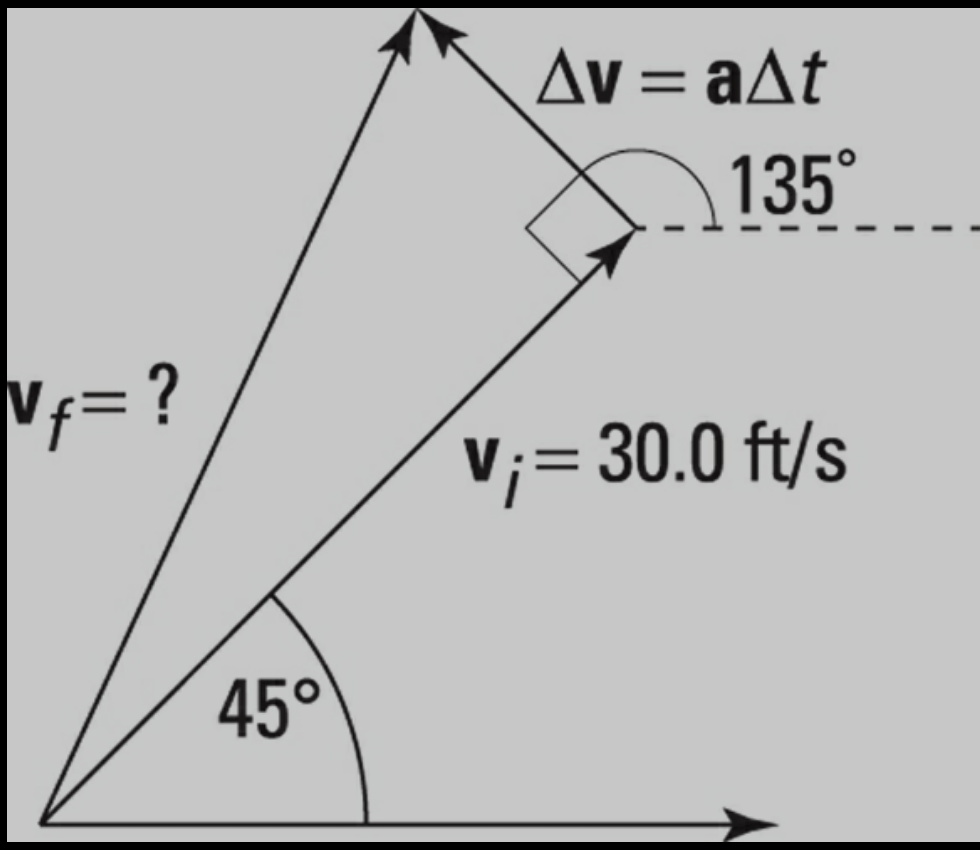
\includegraphics[width=\columnwidth]{image}
\\\\
Holzner, Steven. Physics I For Dummies (For Dummies (Math \& Science)) (p. 68). Wiley. Kindle Edition.
\\\\
\section{Solution}
\[ v=30ft/s \]
\[ \cos(45)=\frac{x}{30} \]
\[ \sin(45)=\frac{x}{30} \]
\[ x=21.2ft/s\ y=21.2ft/s \]
\[ \frac{v_f-(21.2ft/s,21.2ft/s)}{.1s^2}=(\cos(135)*60ft/s^2,\sin(135)*60ft/s^2)\]
\[ v_f-(21.2ft/s,21.2ft/s)=(-4.242ft,4.24ft) \]
\[ v_f=(17.0ft/s,25.4ft/s) \]
\end{document}
